\documentclass[10pt]{beamer}%
 \usetheme[progressbar = foot, background=light, numbering=none]{metropolis} 
 %\usecolortheme[]{owl} %owl-defined colours will be available as OwlRed, OwlGreen, and so forth.
 \setbeamercolor{title separator}{fg=OwlGreen}
%\setsansfont{Ubuntu}
%\setmonofont{Ubuntu Mono}
% % input
% 
\useoutertheme{split}
%\setbeamertemplate{footline}{\small \insertauthor}

\usepackage[utf8]{inputenc}%
 \usepackage{lmodern} %Type1-font for non-english texts and characters
 \usepackage[USenglish]{babel} %francais, polish, spanish, ...
 \usepackage[T1]{fontenc}
% 
 \usepackage{ragged2e}%for text justification by default
 \justifying
% 
 % graphics
 %% Figures %%%%%%%%%%%%%%%%%%%%%%%%%%%%%%%%%%%%%%%%%%%%%%%%%%
 \usepackage{graphicx}
 
 \hypersetup{pdfstartview={Fit}} % fits the presentation to the window when first displayed
 
 \title[https://timotheenivalis.github.io/]{}
 \date{}
 \author[\footnotesize Dr. Timoth\'ee Bonnet ]{ }

%%%%%%%%%%%%%%%%%%%%%%%%%%%%%%%%%%%%%%%%%%%%%%
\begin{document}
% 
% \begin{frame}{Timoth\'ee Bonnet}
% 
% \vfill
% 
\includegraphics[width=0.03\textwidth]{Figures/tweeter.jpeg} @TimotheeBonnet
% \end{frame}
%%%%%%%%%%%
\begin{frame}{Evolutionary quantitative genetics}
   
    \begin{alertblock}{How fast are wild vertebrates evolving? What is selected? How?}
    \centering
        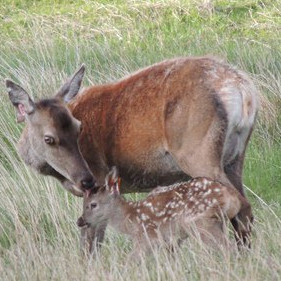
\includegraphics[width=0.15\textwidth]{Figures/doe}
        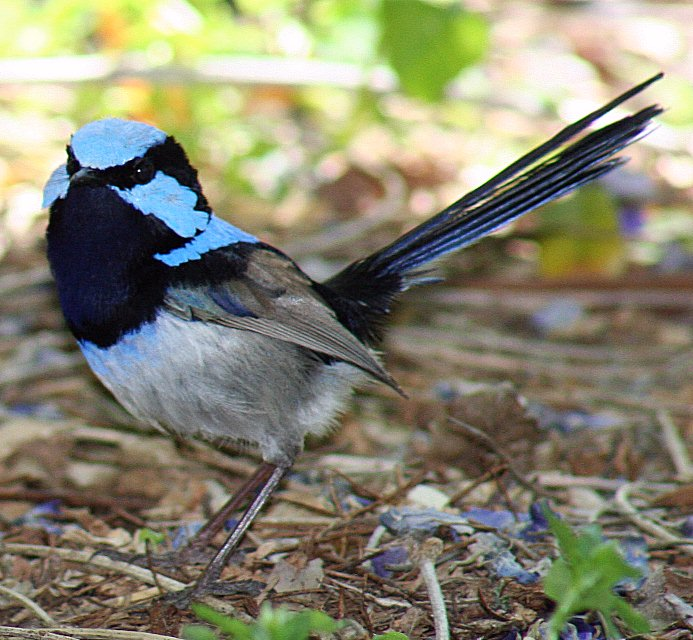
\includegraphics[width=0.15\textwidth]{Figures/sfw}
        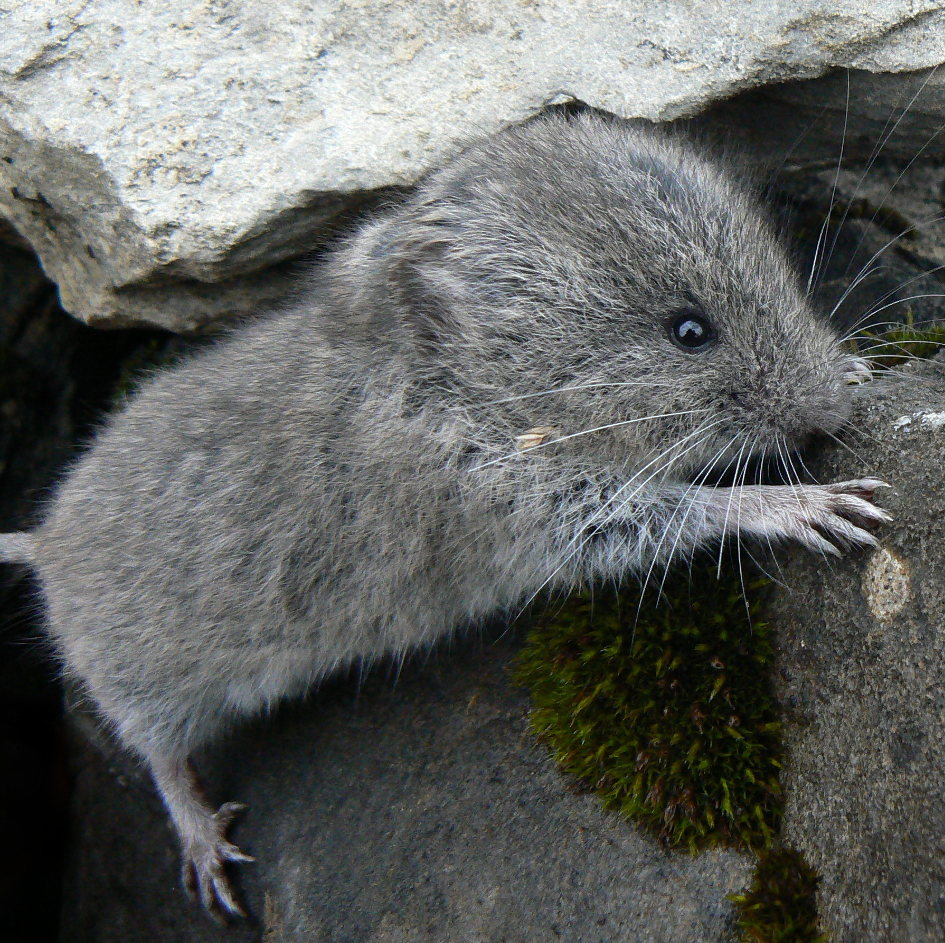
\includegraphics[width=0.15\textwidth]{Figures/vole}
        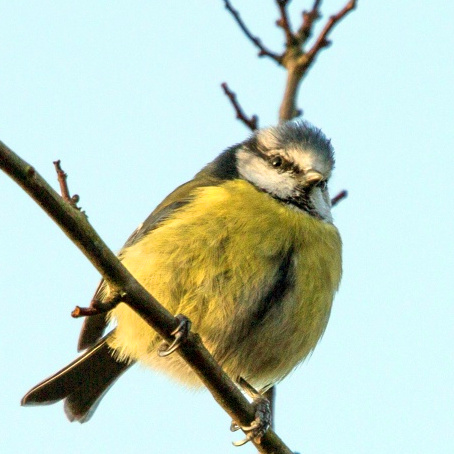
\includegraphics[width=0.15\textwidth]{Figures/bt}
        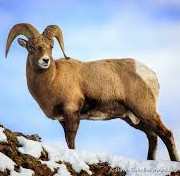
\includegraphics[width=0.15\textwidth]{Figures/bgs}
        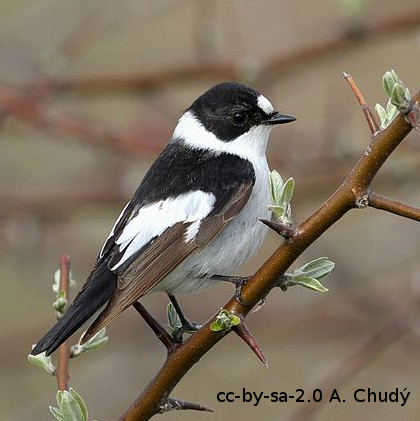
\includegraphics[width=0.15\textwidth]{Figures/cfc}
    \end{alertblock}
    
    \pause
    
    \begin{exampleblock}{When does evolution matter for population dynamics?}
    \centering 
    
\includegraphics[width=0.1\textwidth]{Figures/snowwwvole2}
    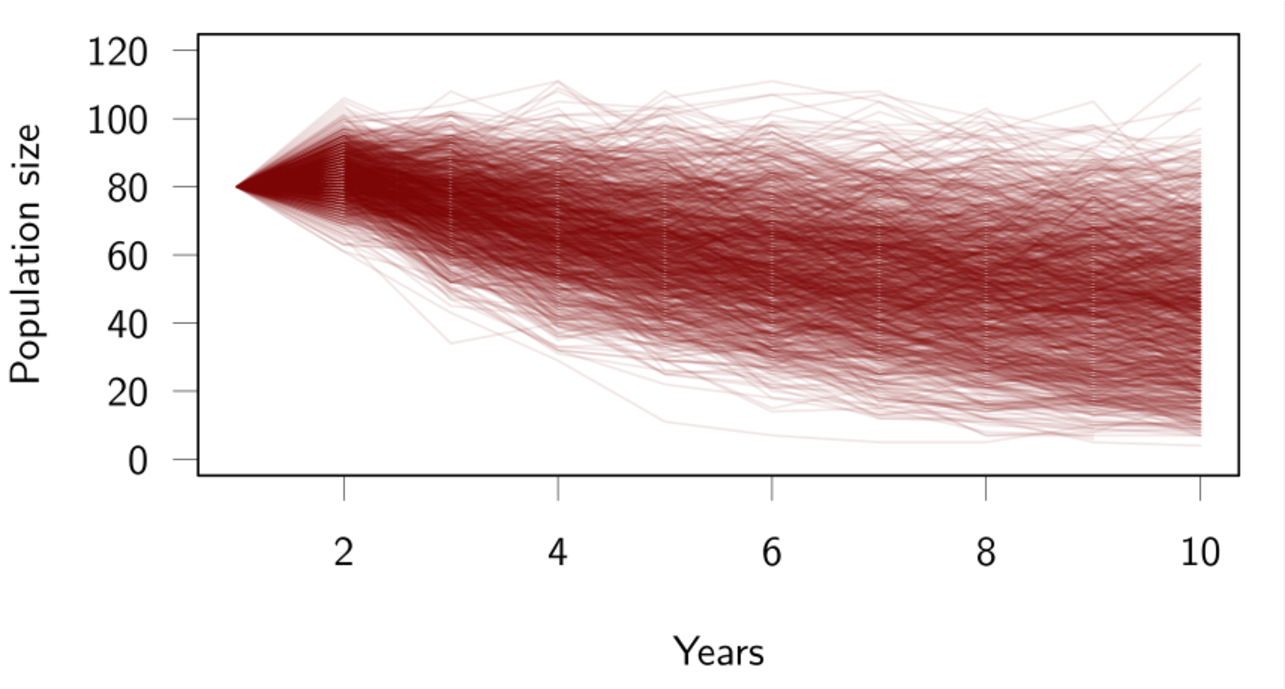
\includegraphics[width=0.4\textwidth]{Figures/stochEx-1}
    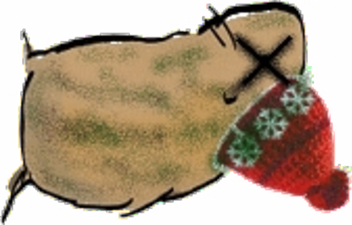
\includegraphics[width=0.15\textwidth]{Figures/Deadsnowwwvole2}
    \end{exampleblock}
    
    \pause
        
    \begin{block}{\color{blue} + various projects \dots}
    \begin{itemize}
     \item Why discordant introgression? Role in current evolution?
     \item Why survival synchronous among bird species at country-scale?
    \end{itemize}
   \end{block}

    
\end{frame}
%%%%%%%%%%%
%%%%%%%%%%%
\begin{frame}{Statistics, coding}
\begin{center}

\includegraphics[width=1\textwidth]{Figures/bdsi}
\textbf{Workshops, courses, consulting\dots}
\end{center}

\begin{columns}[c]
\begin{column}{0.5\textwidth}
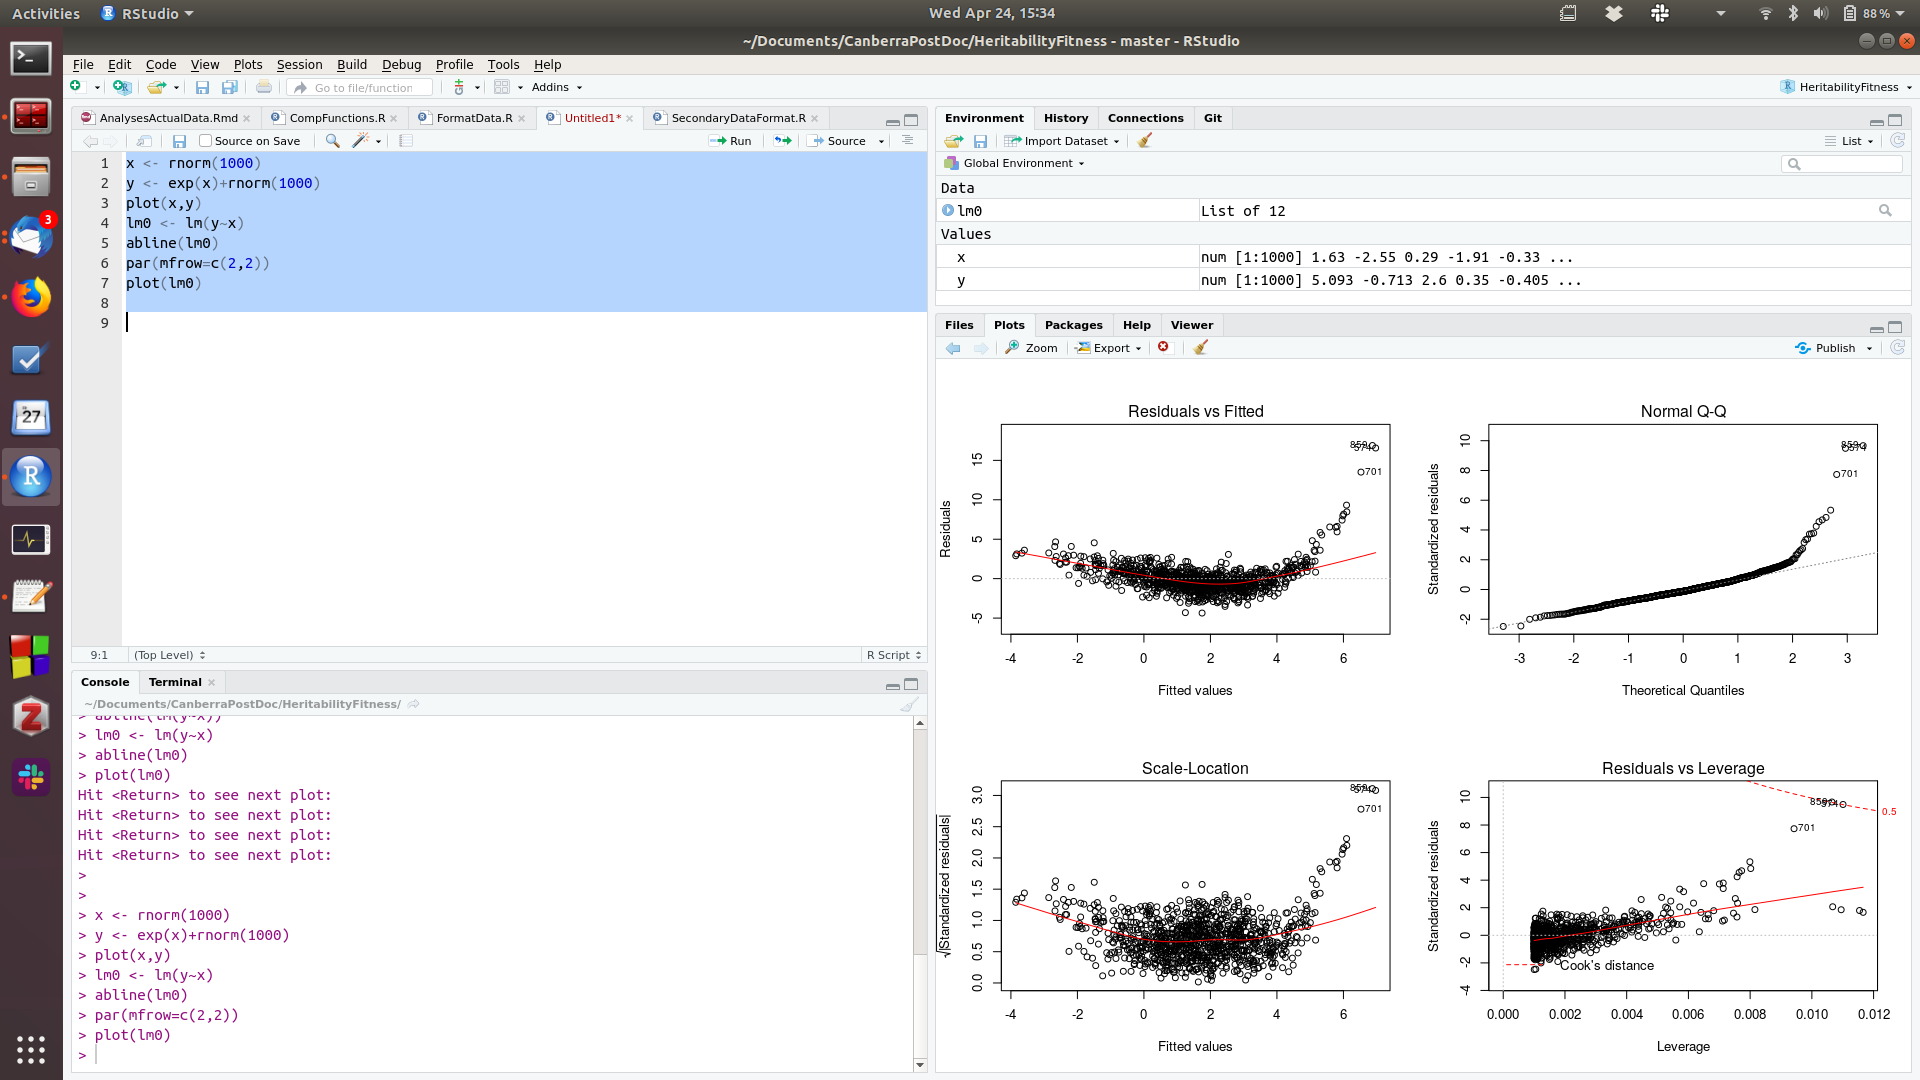
\includegraphics[width=1\textwidth]{Figures/rstudio}
\end{column}
\begin{column}{0.5\textwidth}
    \begin{itemize}
        \item Statistical modelling / inference
        \item R-coding
        \item Computer simulations
        \item (C++, \LaTeX, bash, Git\dots)
    \end{itemize}
\end{column}
\end{columns}

\end{frame}
%%%%%%%%%%%
%%%%%%%%%%%
\begin{frame}{Naturalism}
\begin{tikzpicture} 
    \node (me) at (0,0) {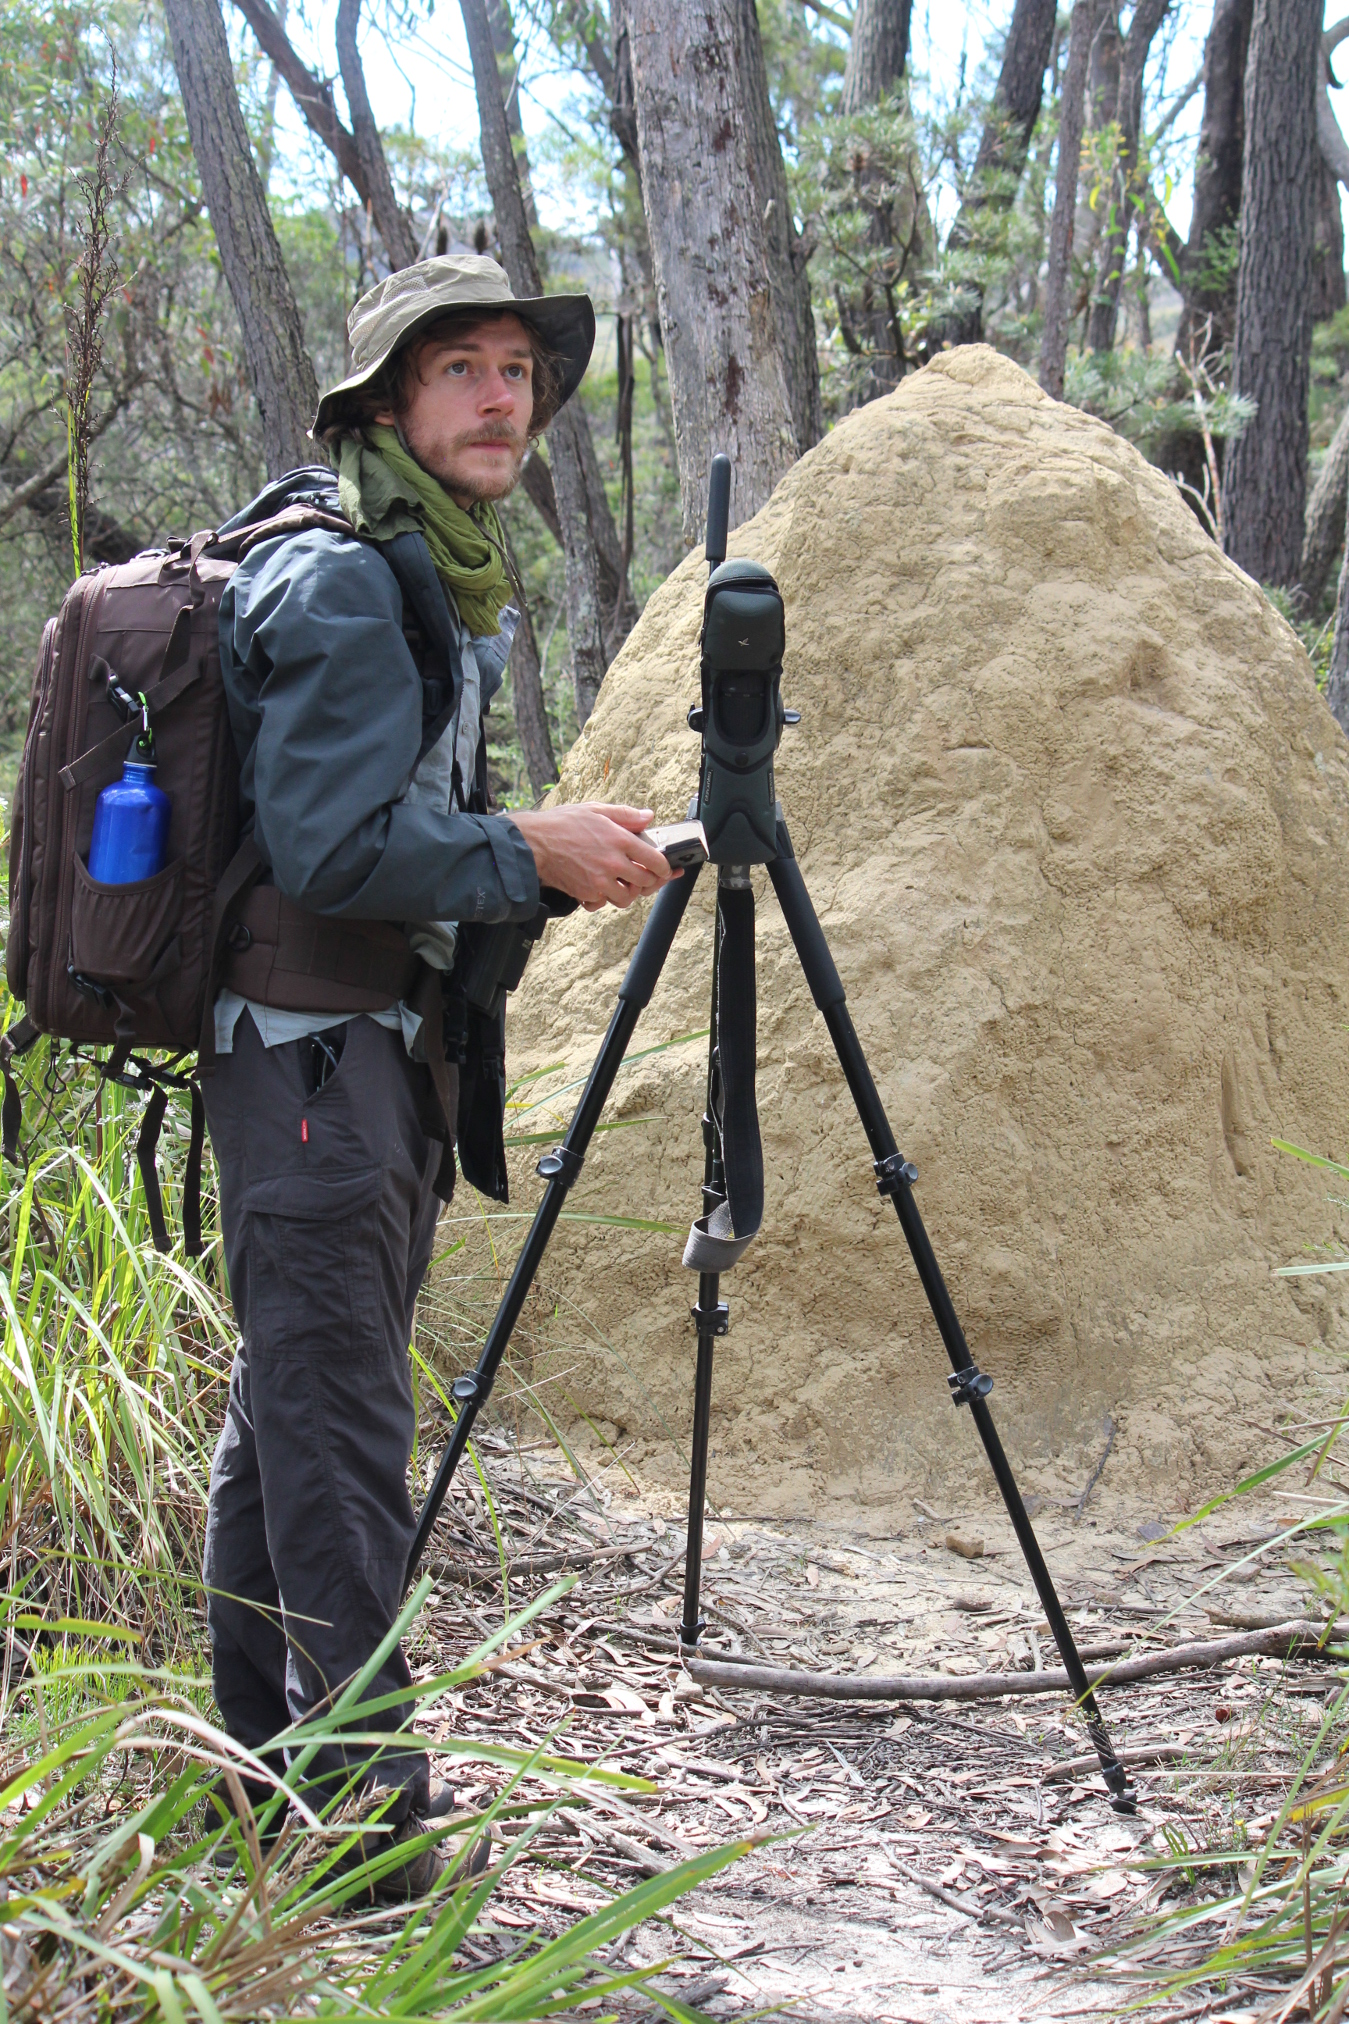
\includegraphics[height=0.8\textheight]{Figures/birding}};
    
    \node[anchor=west] (ld) at (3.5,2) {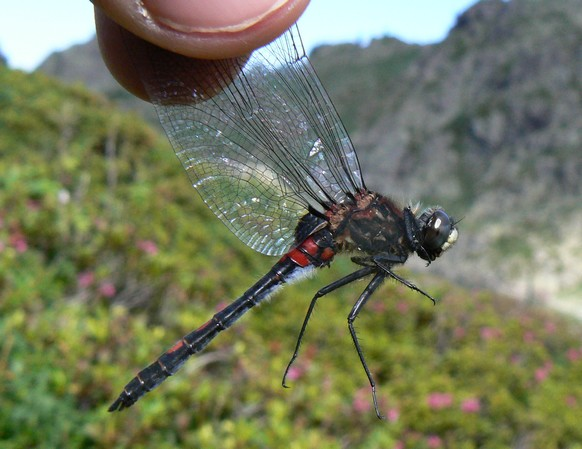
\includegraphics[height=0.3\textheight]{Figures/ld}}; 
        \node[anchor=west] (skull) at (3,-2) {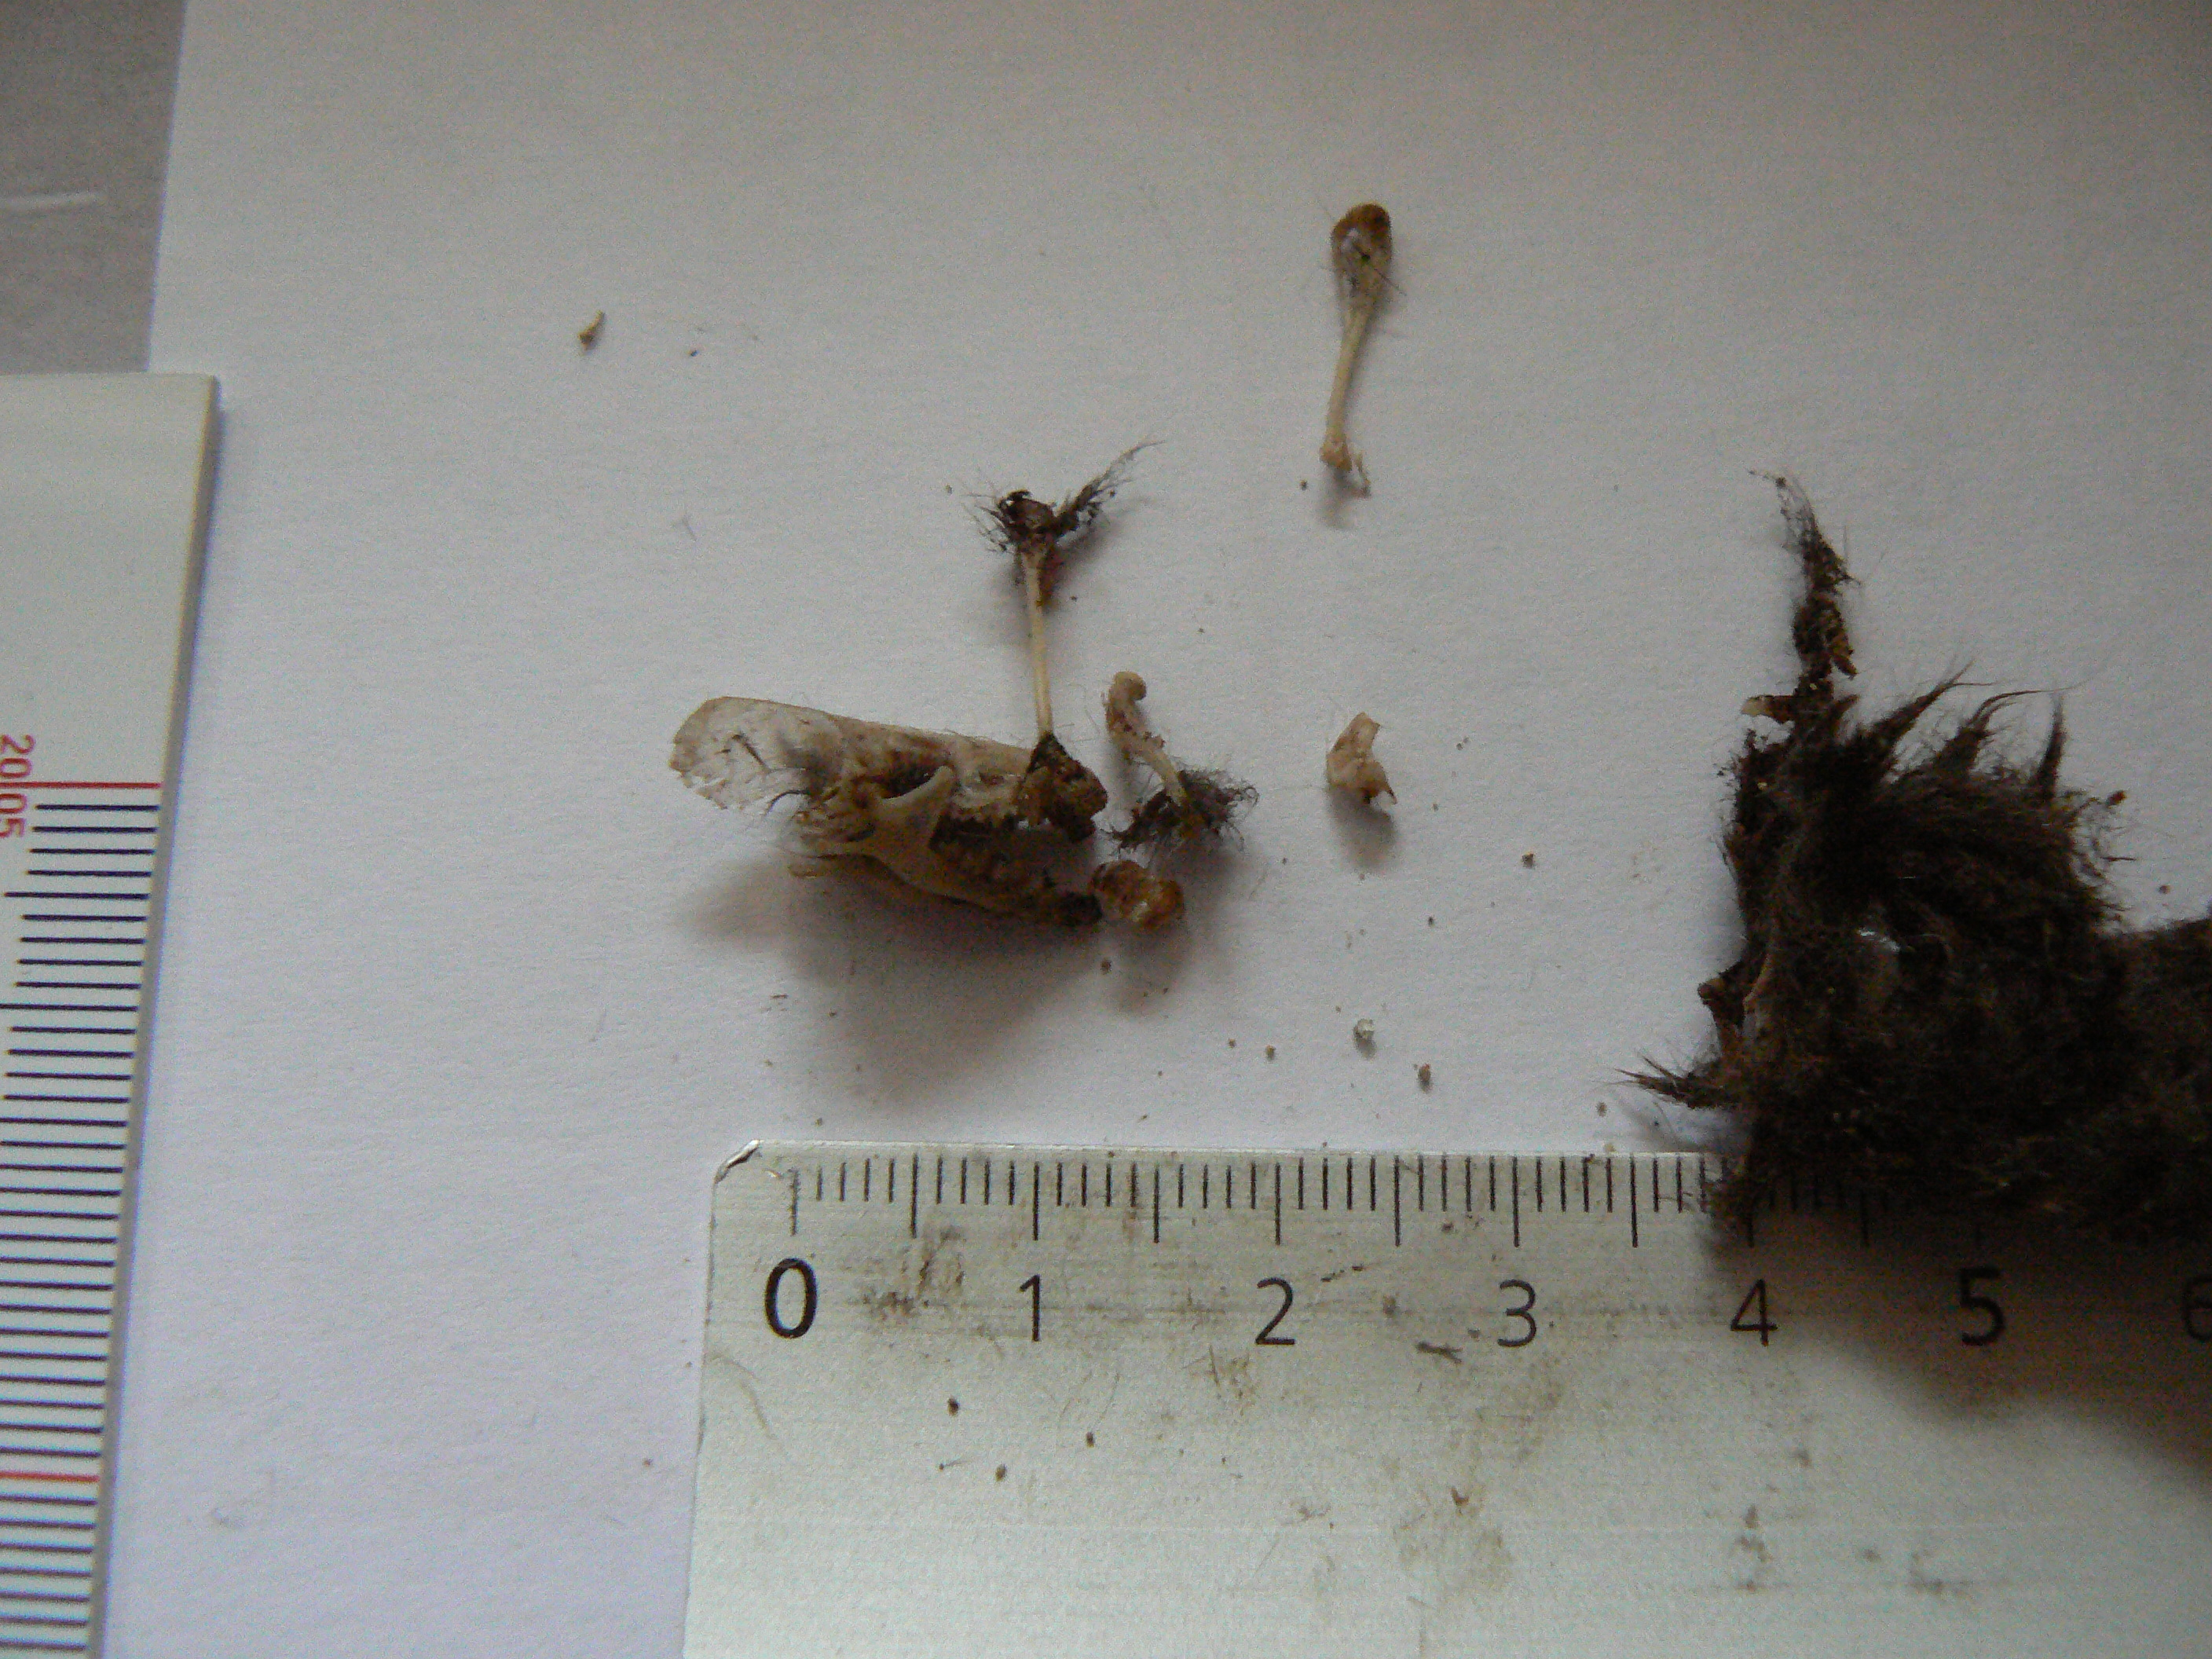
\includegraphics[height=0.3\textheight]{Figures/skull}};
    \node[anchor=west] (colub) at (5,0) {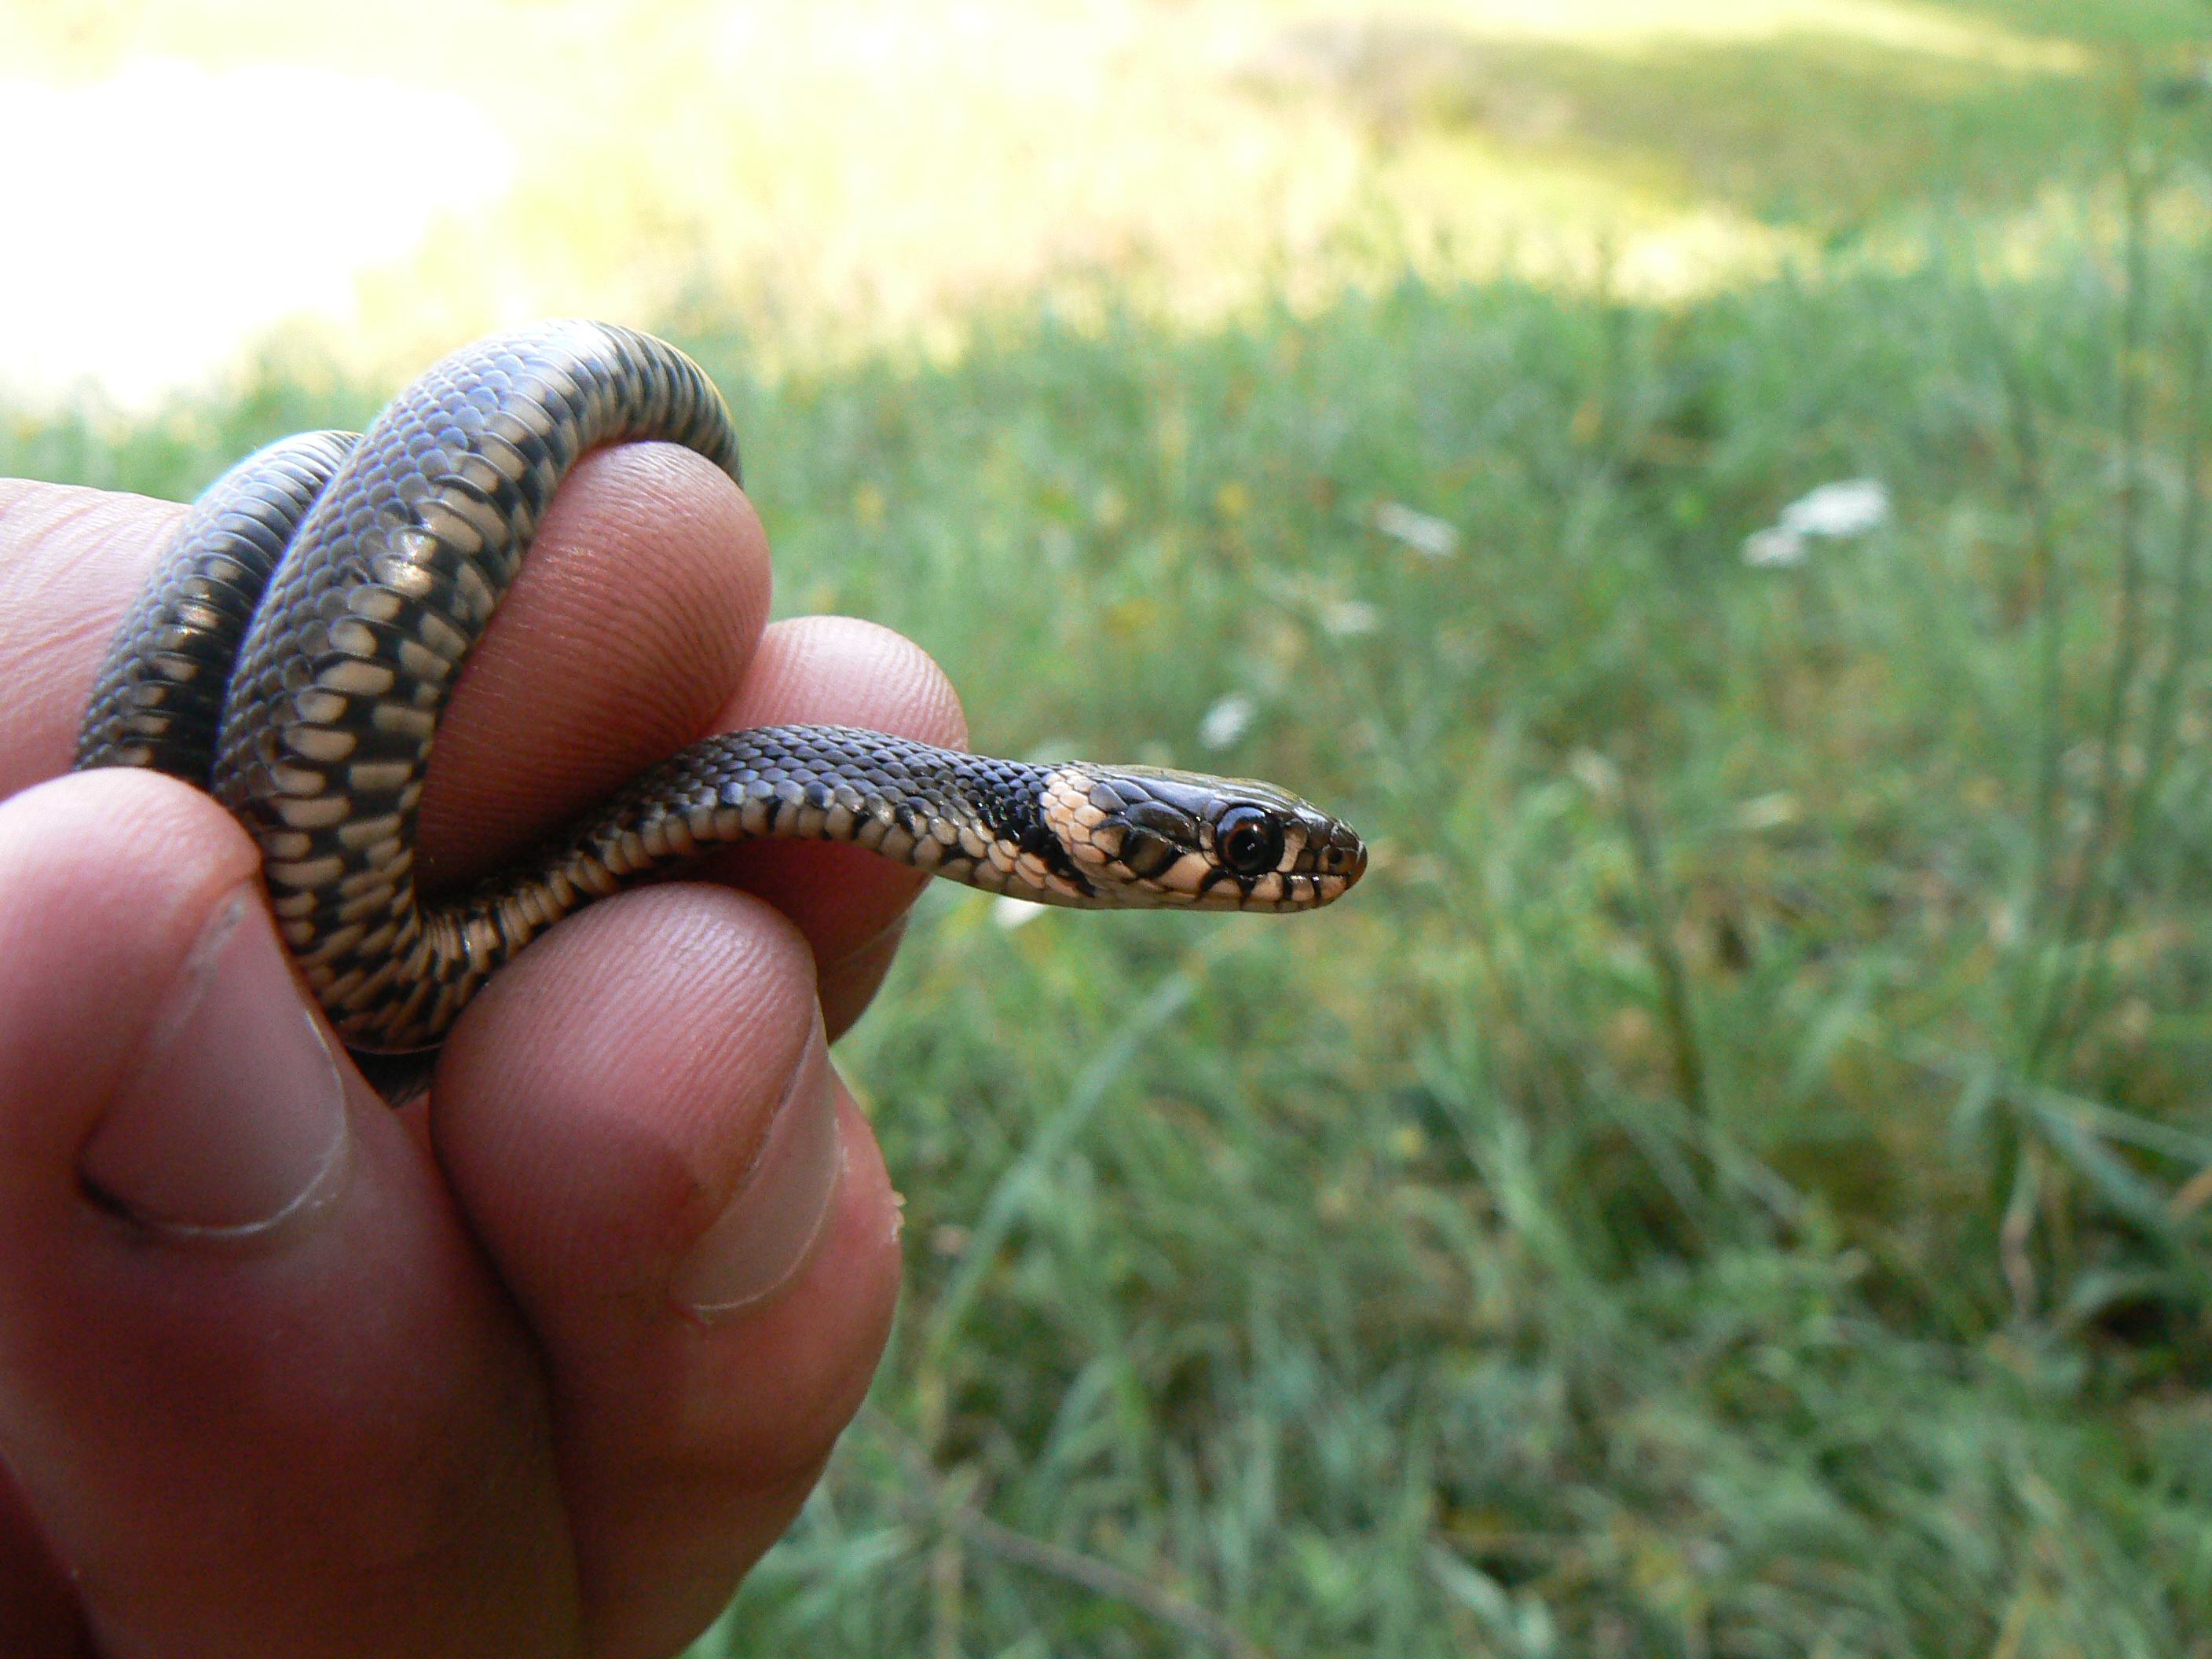
\includegraphics[height=0.25\textheight]{Figures/colub}};
    \node[anchor=west] (ol) at (6,-2.5) {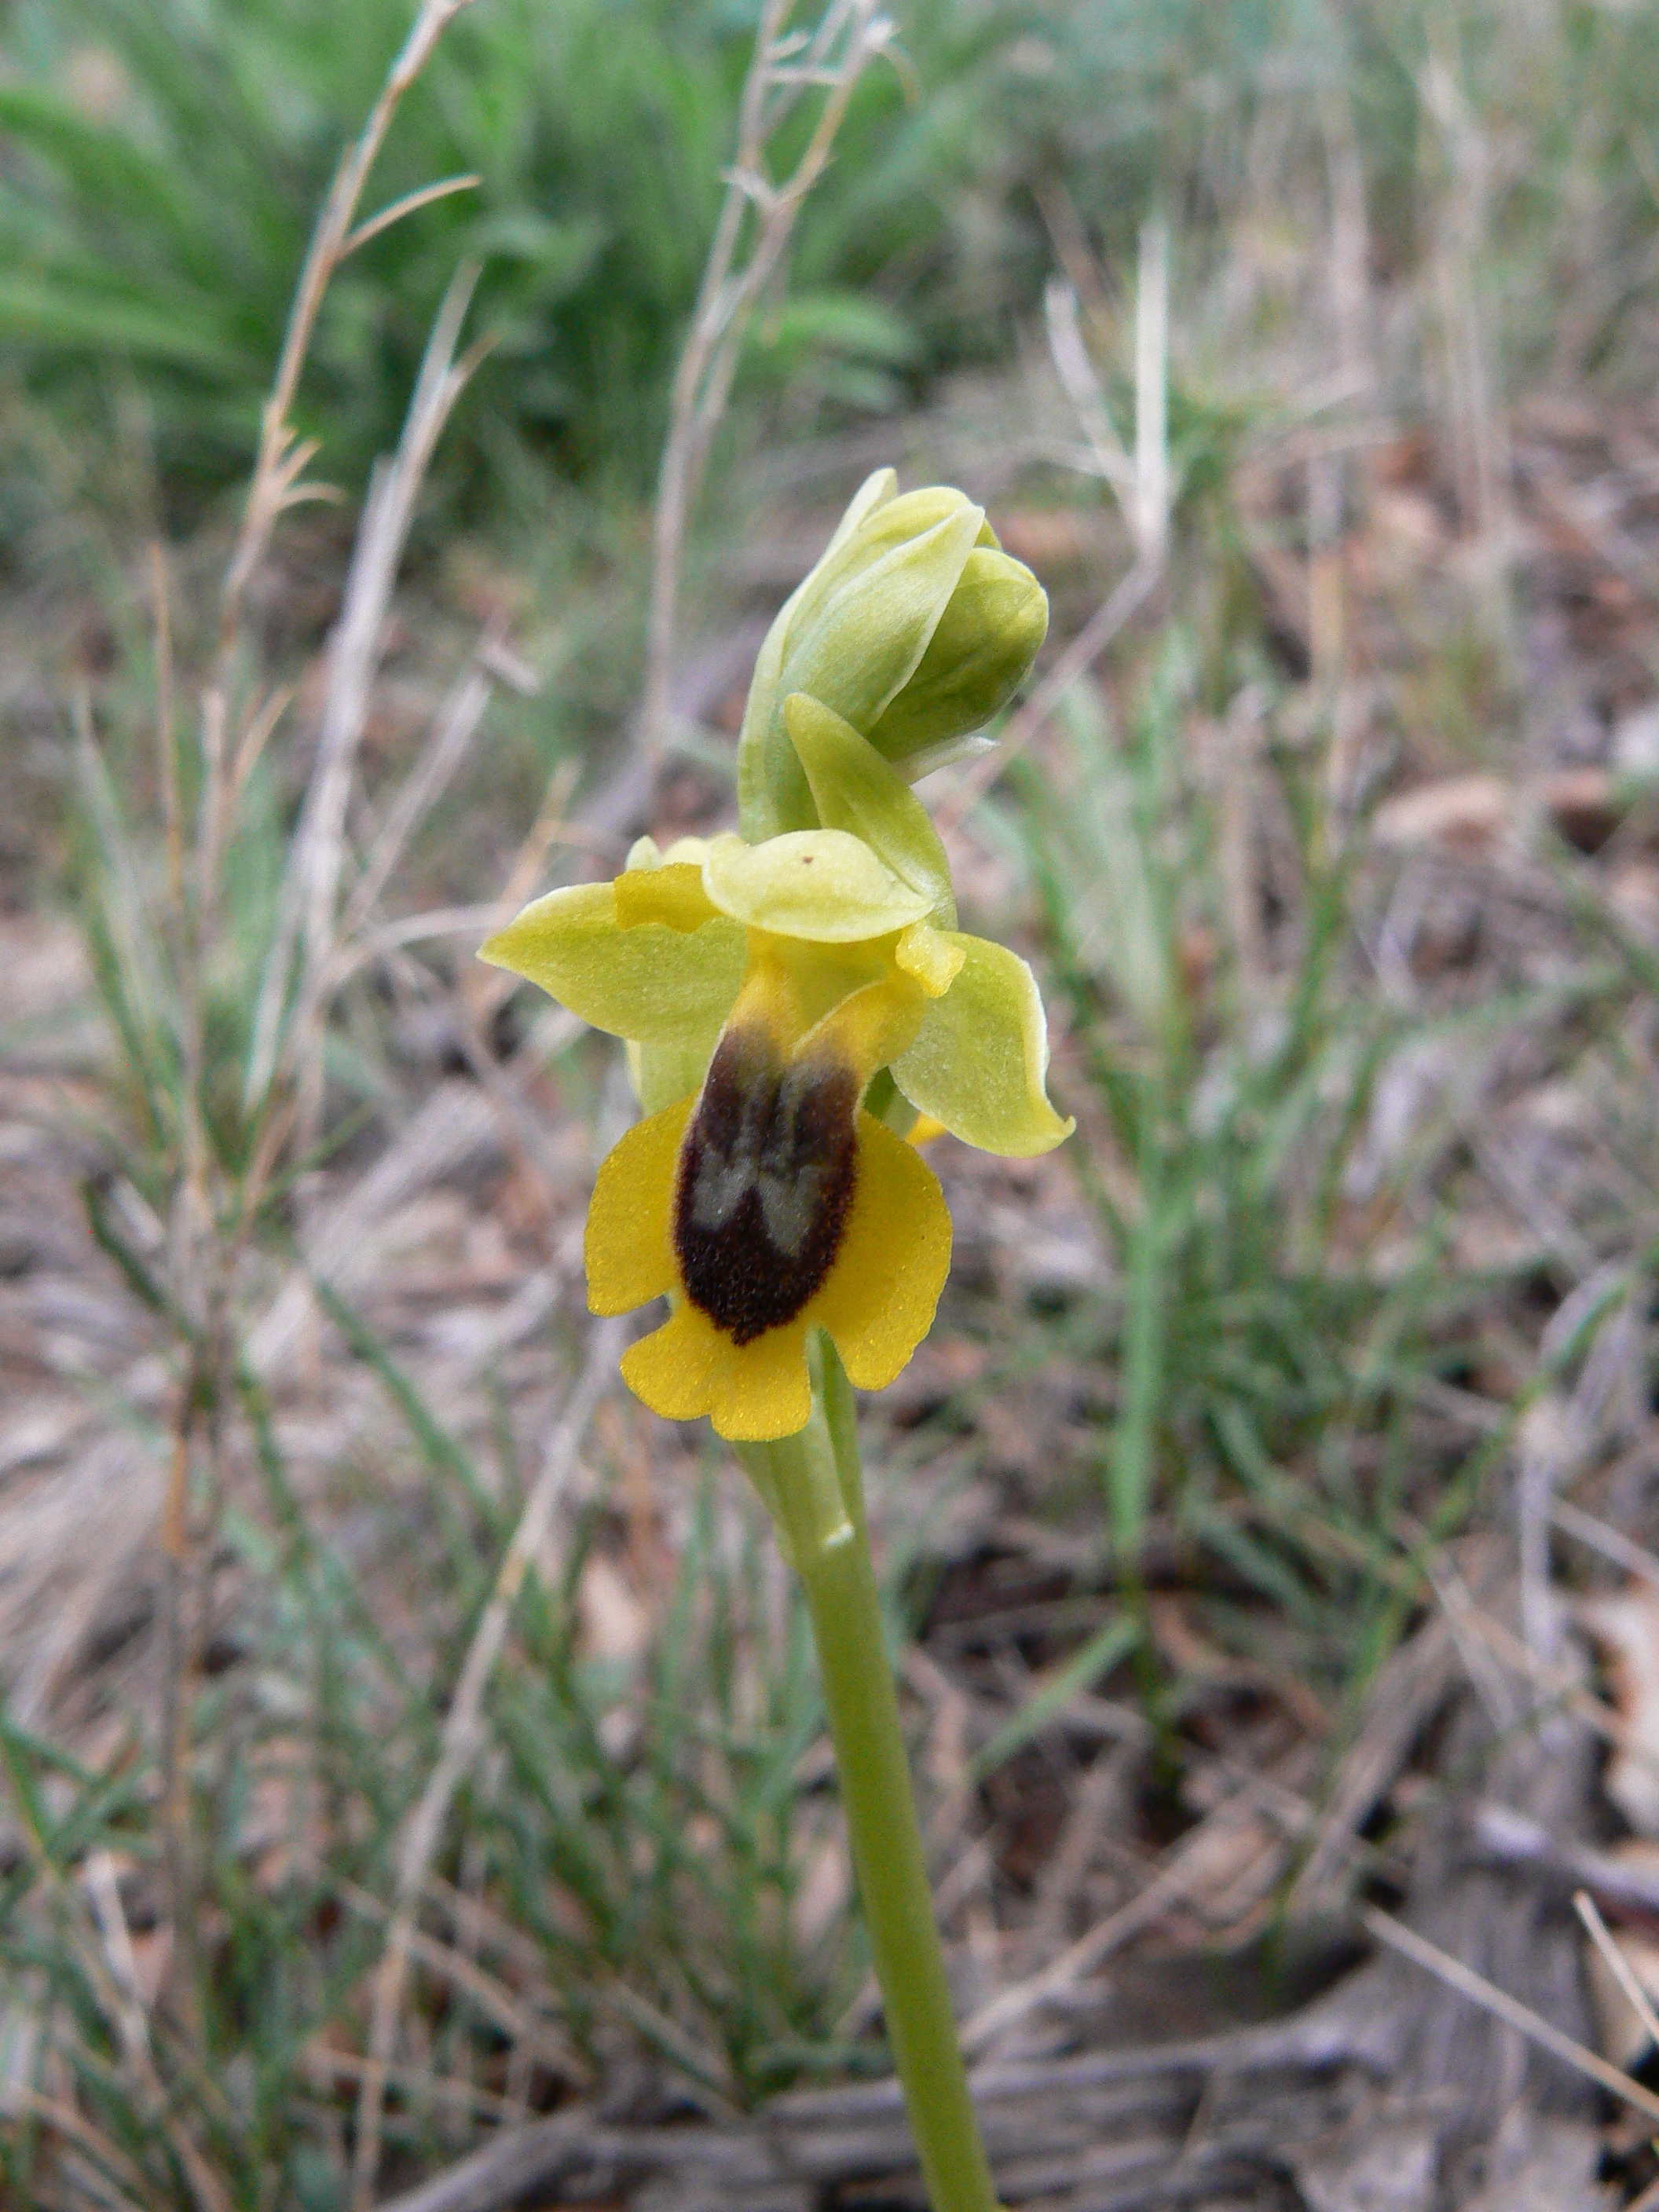
\includegraphics[height=0.3\textheight]{Figures/ol}};
    \node[anchor=west] (cb) at (-0.3,-1.5) {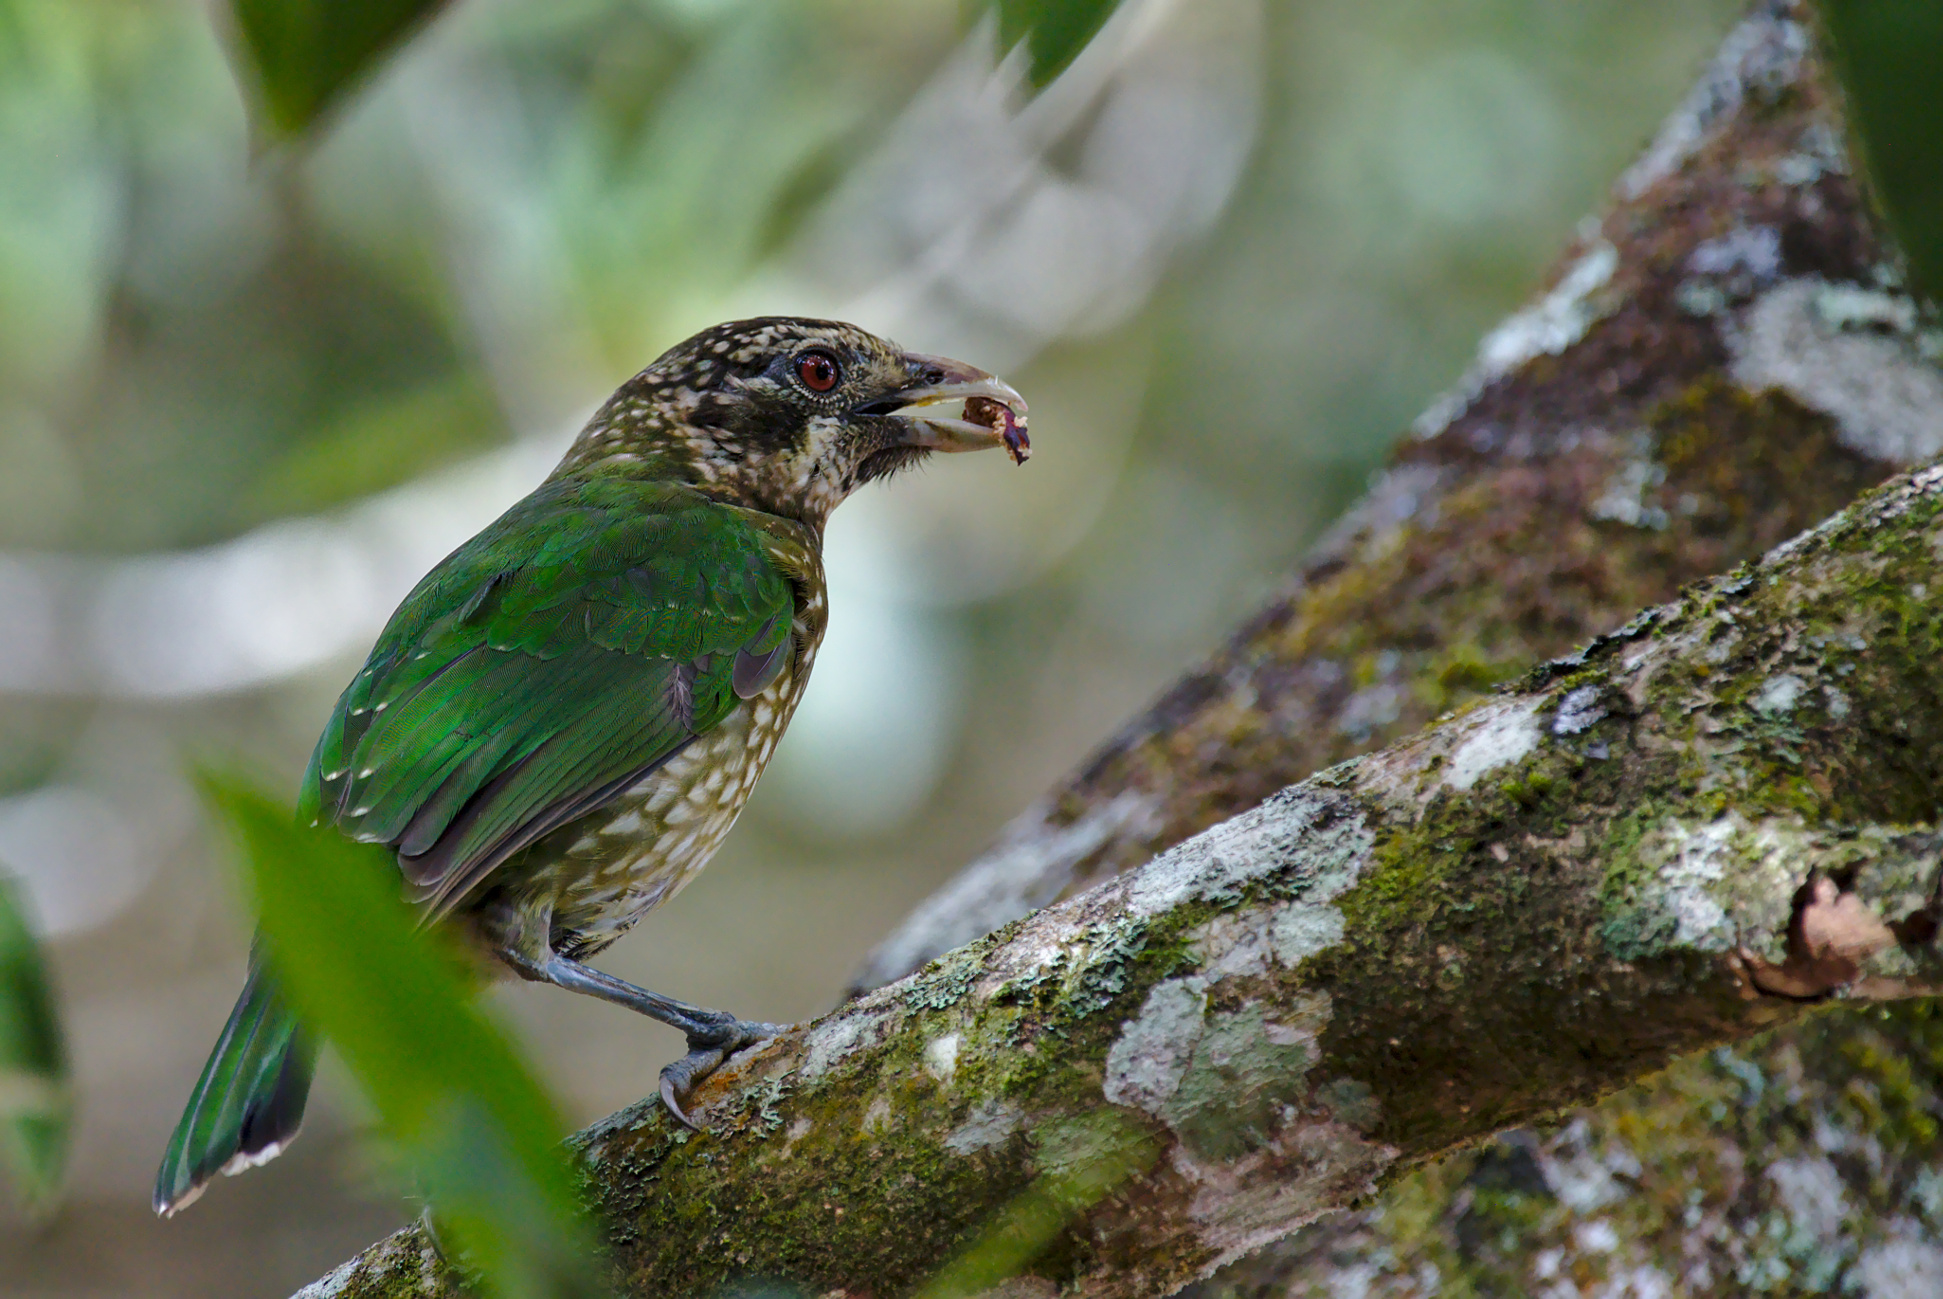
\includegraphics[height=0.3\textheight]{Figures/catb}};
     
\end{tikzpicture}
\end{frame}
%%%%%%%%%%%

\end{document}
